

\makeatletter
\let\@twosidetrue\@twosidefalse
\let\@mparswitchtrue\@mparswitchfalse
\makeatother

\documentclass[10pt,twocolumn]{llncs}
\usepackage[left=2.0cm,right=2.0cm,top=2.5cm,bottom=2.0cm]{geometry}

\typeout{}
\typeout{--------------------------------------------------------------}
\typeout{ +---+ Thesis Template                            }
\typeout{ +---+      Version 2.0, August 2011                         }
\typeout{ +---+  for Instituto Superior Tecnico (IST),                 }
\typeout{ +---+  Universidade T�cnica de Lisboa                         }
\typeout{ * Using Thesis Style form Pedro Tom�s                                }
\typeout{ * Created to write Dissertations                             }
\typeout{ * Conforms with IST Master Degree format and with most important packages setup        }
\typeout{ * Should conform with IST PhD Degree format (not verified)   }
\typeout{                                                              }
\typeout{ AUTHOR: Miguel Amador and Jo�o Marques                                          }
\typeout{                                                              }
\typeout{Important: Use all files in the archive, since this is based in all them. Modify dummy files at wish.                                                              }
\typeout{--------------------------------------------------------------}
\typeout{}

% Defines an additional alphabet... not required in most cases
% ------------------------------------------------------------
% \DeclareMathAlphabet{\mathpzc}{OT1}{pzc}{m}{it}

% PACKAGE babel:
% ---------------
% The 'babel' package may correct some hyphenisation issues of latex. 
% However in most situations it is not required.
\usepackage[english]{babel}

% PACKAGE fontenc:
% -----------------
% chooses T1-fonts and allows correct automatic hyphenation.
%\usepackage[T1]{fontenc}
\usepackage[latin1]{inputenc}
%\usepackage[utf8]{inPUTenc}									% UTF 8, Caracteres ocidentais

% PACKAGE eurosym:
% -----------------
% allows the use of the european currency sign
\usepackage{eurosym}

% PACKAGE lettrine:
% -----------------
% allows the use of drop cap lettering
\usepackage{type1cm}
\usepackage{lettrine}

% Package ulem.
\usepackage{ulem} % Allows the use of other text emphatizer commands
\normalem %defines \emph{} to italic, instead of underline. 
\raggedbottom %declaration makes all pages the height of the text on that page. No extra vertical space is added. The \flushbottom declaration makes all text pages the same height, adding extra vertical space when necessary to fill out the page.

% PACKAGE date time:
% -----------------
% Lets you alter the format of the date that \today returns.
\usepackage{datetime}
\newdateformat{todaythesis}{%
\monthname[\THEMONTH]  \THEYEAR}

% PACKAGE latexsym:
% -----------------
% Defines additional latex symbols. May be required for thesis with many math symbols.
\usepackage{latexsym}

% PACKAGE amsmath, amsthm, amssymb, amsfonts:
% -------------------------------------------
% This package is typically required. Among many other things it adds the possibility
% to put symbols in bold by using \boldsymbol (not \mathbf); defines additional 
% fonts and symbols; adds the \eqref command for citing equations. I prefer the style
% "(x.xx)" for referering to an equation than to use "equation x.xx".
\usepackage{amsmath, amsthm, amssymb, amsfonts, amsbsy}

% PACKAGE multirow, colortbl, longtable:
% ---------------------------------------
% These packages are most useful for advanced tables. The first allows to join rows 
% through the command \multirow which works similarly with the command \multicolumn
% The second package allows to color the table (both foreground and background)
% The third package is only required when tables extend beyond the length of one page;
% with compatibilities with the tabular environment. The last allow the definitions of landscape pages, allowing the use of a different orientation for wider graphics or tables. See package documentation to see the implementation.
\usepackage{multirow}
\usepackage{colortbl}
\usepackage{supertabular}
\usepackage{pdflscape}
% \usepackage{longtable}

% PACKAGE graphics, epsfig, subfigure, caption:
% ---------------------------------------------
% Packages for figures... well you will certainly need these packages, with the exception
% of the 'caption' package. This only allows to define extra caption options.
% Notice that subfigure allows to place figures within figures with its own caption. It
% should be avoided to create an eps file with subfigures. That will mean that you won't be 
% able to reference those subfigures. Instead create an EPS file (the only graphics format supported
% by latex) for each of the subfigures and then use the command \subfigure (see below).
\usepackage{graphics}
\usepackage{graphicx}
\usepackage{epsfig}
\usepackage[hang,small,bf]{subfigure}
%\usepackage[footnotesize,bf,center]{caption}
\usepackage{dcolumn}
\usepackage{bm}
\usepackage{booktabs}
\usepackage{rotating}
\usepackage{multirow}

\usepackage[font=small,labelfont=bf,textfont=normalfont]{caption}

% PACKAGE algorithmic, algorithm
% ------------------------------
% These packages are required if you need to describe an algorithm.
% \usepackage{algorithmic}
% \usepackage[chapter]{algorithm}

% PACKAGE natbib/cite
% -------------------
% The two packages are not compatible, and you should use one of the two. Notice however that the
% IEEE BiBTeX stylesheet is imcompatible with the natbib package. If using the IEEE format, use the 
% cite package instead
%\usepackage[square,numbers,sort&compress]{natbib}
\usepackage{cite}

% PACKAGE acronym
% -----------------
% This package is most useful for acronyms. The package guarantees that all acronyms definitions are 
% given at the first usage. IMPORTANT: do not use acronyms in titles/captions; otherwise the definition 
% will appear on the table of contents.
\usepackage[printonlyused]{acronym}
\usepackage[titletoc,title,header]{appendix}
\usepackage[noauto]{chappg}

% PACKAGE extra_functions
% -----------------
% My Personal package: defines the following commands:
% \fancychapter{chaptername) -> Prints a fancier chapter (you can also use the fancychapter package for this)
% \hline{width} -> use for a replacement of the \hline command
% \Mark1, \Mark2, \Mark3, ...
\usepackage{00.extra_functions}


% PACKAGE hyperref
% -----------------
% Set links for references and citations in document
% Some MiKTeX distributions have faulty PDF creators in which case this package will not work correctly
% Long live Linux :D
\usepackage[plainpages=false]{hyperref}
\hypersetup{
             colorlinks=false,
             citecolor=red,
             breaklinks=true,
             bookmarksnumbered=true,
             bookmarksopen=true,
             pdftitle={Benchmark Kinect},
             pdfauthor={Jo�o Pedro Ribeiro Machado},
             pdfsubject={Master Thesis in Information Systems and Computer Engineering},
             pdfcreator={TeXstudio},
             pdfkeywords={Template, Latex, Thesis}}
\usepackage{float}
%\usepackage[final]{00.listofsymbols}
\usepackage{00.symlist}

% Set paragraph counter to alphanumeric mode
\renewcommand{\theparagraph}{\Alph{paragraph}~--}

\newcommand{\figref}[1]{Figure \ref{#1}}
\newcommand{\equationref}[1]{Equation (\ref{#1})}
\newcommand{\tableref}[1]{Table (\ref{#1})}

\newcommand{\textreg}{$\textsuperscript{\textregistered}$}


% MINE MINE
\newcounter{eqn}
\renewcommand*{\theeqn}{\alph{eqn})}
\newcommand{\num}{\refstepcounter{eqn}\text{\theeqn}\;}

\makeatletter
\newcommand{\putindeepbox}[2][0.7\baselineskip]{{%
    \setbox0=\hbox{#2}%
    \setbox0=\vbox{\noindent\hsize=\wd0\unhbox0}
    \@tempdima=\dp0
    \advance\@tempdima by \ht0
    \advance\@tempdima by -#1\relax
    \dp0=\@tempdima
    \ht0=#1\relax
    \box0
}}
\makeatother


% MINE MINE



% load package with ``framed'' and ``numbered'' option.
\usepackage[framed,numbered,autolinebreaks,useliterate]{mcode}

% something NOT relevant to the usage of the package.
\setlength{\parindent}{0pt}
\setlength{\parskip}{18pt}
\title{\texttt{mcode.sty} Demo}
\author{Florian Knorn, \texttt{florian@knorn.org}}
% //////////////////////////////////////////////////



%% Title
\title{Quantum Pirates} % use \\ if the title is too big
\subtitle{A Quantum Game-Theory Approach to The Pirate Game}

%% Author \inst{1}
\author{Daniela Fontes}
% \thanks{\email{daniela.fontesl@ist.utl.pt}
%% Institute, mails and websites
\institute{	
		Instituto Superior T\'ecnico
\\
\email{daniela.fontesl@ist.utl.pt}
}



\begin{document}

	\maketitle

	\begin{abstract}
		In this document, we develop a model and a simulation of a quantization scheme for the mathematical puzzle created by Omohundro and Stewart - ``A puzzle for pirates '', also known as Pirate Game. This game is a multi-player version of the game ``Ultimatum '', where the players (Pirates), must distribute fixed number of gold coins acording to some rules.

		\keywords Quantum Game Theory; Pirate Game; Quantum Mechanics; Quantum Computing; Game Theory; Probability Theory

\end{abstract}

\section{Introduction}




\section{Pirate Game}
\label{sec:pirate_description}

The original Pirate Game is a multi-player version of the Ultimatum game that was first published as a mathematical problem in the Scientific American as a mathematical problem posed by Omohundro\cite{Stewart1999}. The problem can be formulated as it follows:

\begin{quotation}
Suppose there are 5 rational pirates: A; B; C; D; E. The pirates have a  loot of 100 indivisible gold coins to divide among themselves.


As the pirates have a strict hierarchy, in which pirate A is the captain and E has the lowest rank, the highest ranking pirate alive will propose a division. Then each pirate will cast a vote on whether or not to accept the proposal. 

If a majority or a tie is reached the goods will be allocated according to the proposal. Otherwise the proposer will be thrown overboard and the next pirate in the hierarchy assumes the place of the captain. 

We consider that each pirate privileges her survival, and then will want to maximize the number of coins received. When the result is indifferent the pirates prefer to throw another pirate overboard and thus climbing in the hierarchy. 
\end{quotation}

\subsection{Analysis of the Pirate Game for $3$ Players}
\label{subsubsec:analysis_PG3players}

In Figure \ref{fig:pg_architecturegametree:extensiveform} we have an extensive form representation of the classic Pirate Game for $3$ players without taking into account the proposals. Each node in the game tree has the number of the player who will make the decision, either to Cooperate (vote yes to the proposal), or Defect. 

\begin{figure}[h]
\centering 
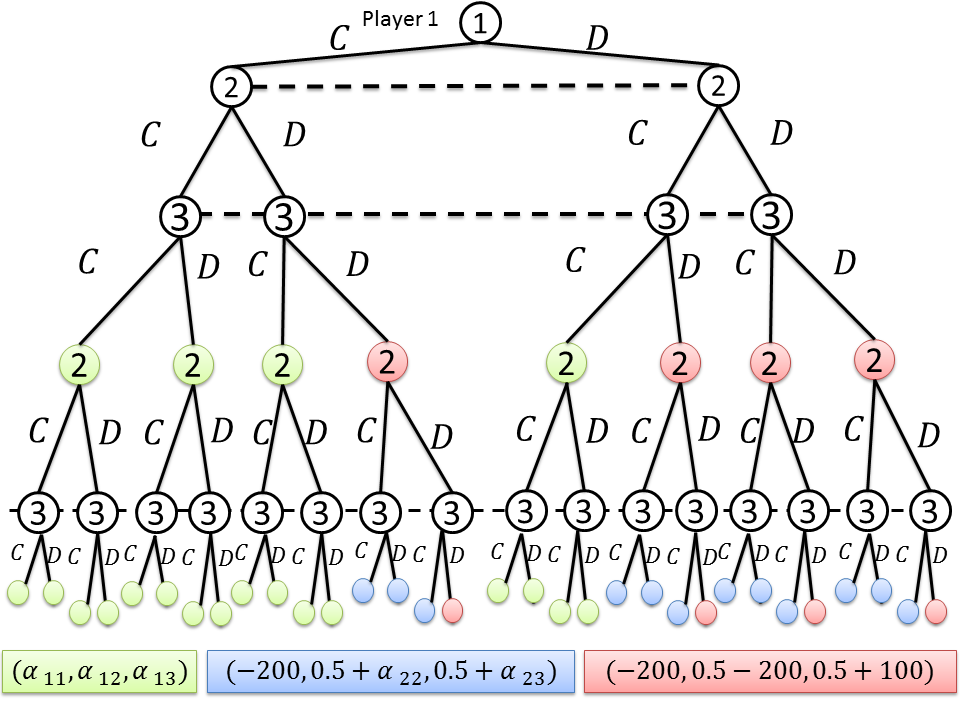
\includegraphics[scale=0.28]{Figures/1.5qubit/FigurasRevistas/Slide1.png}
\caption{Extensive form representation of the classic Pirate Game for $3$ players. }
\label{fig:pg_architecturegametree:extensiveform}
\end{figure}

The green accent, in Figure \ref{fig:pg_architecturegametree:extensiveform}, shown in the nodes represent a state where the first captain (player $1$), will see her proposal accepted, the utility associated. The dashed lines are a common representation for imperfect information  at the nodes united. The blue accent denotes the outcomes where the second captain makes a proposal and has seen it accepted. The red accent color represents the outcomes where the player $3$ will be the remaining pirate.

The number of coins will translate directly the utility associated receiving them. The highest ranking pirate in the hierarchy is responsible to make a proposal to divide the 100 gold coins. A captain $i$ chooses the amount of coins a player $j$ get; this amount will be represented by $\alpha_{ij}$. In the initial stage of the game the captain will define $\alpha_{11}, \alpha_{12}, \alpha_{13}$, according to Equation \ref{eq:goodss} ($N$ the number of pirates in the game). To account for all possible proposals $\alpha_{ij}$ would be overwhelming from the point of the game tree, and from the formulation of the problem the pirates know the share proposal before voting. This means we will concentrate our analysis in the voting aspect. This means that for each specification of the values $\alpha_{ij}$ we will have a diferent game. 

\begin{equation}
\label{eq:goodss}
\forall i \in \{1 , 2, ..., N-1\} : \sum_{j=i}^{N}\alpha_{ij}=100, \forall i,j :\alpha_{ij}\in\mathbb{N}_{0}
\end{equation}

The values for $(\alpha_{11}, \alpha_{12}, \alpha_{13})=(99, 0, 1)$ will be the allocation that results in an equilibrium for the $3$ player game. 


If the proposal is rejected the captain will be thrown off board, and the captain he will receive a negative payoff of $-200$. The pirates have also an incentive to climb the hierarchy; accounted by adding an expected value of half a coin ($0.5$), to the payoff of the remaining players if the voting fails. This tie breaker and death penalty is shown in Figure \ref{fig:pg_architecturegametree:extensiveform}.

\section{Quantum Model}
\subsection{Game system: Setting up the Initial State}
\label{subsec:pirates_initialstate}

A game $\Gamma$ can be viewed as a system composed by qubits manipulated by players. We will use the definition of quantum game proposed by \cite{Fra2011a}, to model extensive form games in a normal form representation. Akin to the Quantum Ultimatum game desbribed in \cite{Fra2011}, our objective is to apply that quantization scheme to the normal form representation of the game tree in Figure \ref{fig:pg_architecturegametree:extensiveform}. 

The representation assumes that each qubit, as in the equation bellow, can be manipulated to represent an action. The pure basis $\vert 0\rangle = \vert C\rangle$ (``C'' from ``Cooperate''), and $\vert 1\rangle = \vert D\rangle$ (``D'' from ``Defect''), representing a yes/no decision or a cooperate/defeat as
those found in many classical game theory problems.

\begin{equation}
\varphi = \alpha . \vert C \rangle + \beta . \vert D \rangle, \{ \alpha ,\beta \} \in \mathbb{C} : \alpha^2 + \beta^2 =1
\end{equation}

A game in this
form is represented by the following a six-tuple:
\begin{equation}
\Gamma=(\mathcal{H}^{2^{a}},\: N,\:\vert\psi_{in}\rangle,\:\xi,\:\{\mathcal{U}_{j}\},\:\{E_{i}\})\label{eq:quantum_game_six_tuple}
\end{equation}


\subsubsection{Actions} $a$ is the number of actions (qubits), in the game. In this $3$ player game there will be $5$ qubits $\varphi_{j}$, as shown bellow, representing the actions or the players decision; three qubits will represent the first voting round, the other two will portray the actions of the second voting round. 

\begin{equation}
\begin{split}
\varphi_{j} = a . \vert C \rangle + b . \vert D \rangle , \\  j \in \{ 1, 2, 3, 4, 5 \}, \\ \{ a,b \} \in \mathbb{C} : a^2 + b^2 =1
\end{split}
\label{eq:opvarphiquantumstates}
\end{equation}

The number of qubits needed to represent the game grows exponentially with the number of players. For $N$ players we need $\sum_{i=2}^{N}{i}$ qubits. With 8 players, this game would already be impractical to simulate in a classical computer. In this regard a quantum computer may enhance our power to simulate this kinds of experiments \cite{Rieffel2011}; 

\subsubsection{Game Space} $\mathcal{H}^{2^{a}}$ is a $2^{a}$-dimensional Hilbert space constructed
as $\otimes_{j=1}^{a}\mathbb{C}^{2}$, with basis $\mathcal{B}$. With $3$ players and $5$ actions our system with be represented in a $\mathcal{H}^{32}$ using a state $\psi$. This means that to represent our system we will need $2^{5}\times 1$ vectors, our system grows exponentially with the number of players/qubits. Each pure basis  of $\mathcal{H}^{32}$ will represent a possible outcome in the game;

\subsubsection{Initial State} $\vert\psi_{in}\rangle$ is the initial state of the compound-system
composed by $a$ qubits: $\vert\varphi_{1}\rangle,\:\vert\varphi_{2}\rangle, ..., \vert\varphi_{j}\rangle, ..., \vert\varphi_{a}\rangle$.

Our initial system ($\vert \psi_{0}(\gamma) \rangle$), will be set up by defining an entanglement coefficient $\gamma$, that affect the way the five qubits (belonging to the three pirate players), are related; this is shown in Equation \eqref{eq:estado_inicial_pg}. 
We will entangle our state by applying the gate $\mathcal{J}$ \cite{Letters2002}. This gate was chosen to accomodate the classical version where players play only classical strategies because in the classical setting there is no entanglement. This is accomplished by chosing $\mathcal{J}$ such that it commutes with any combination of pure strategies (for example $ [ \mathcal{J} , D \otimes C \otimes D \otimes D \otimes C ] = 0 $)

The parameter $\gamma$ becomes a way to measure the entanglement in the system\cite{Eisert2008}. 

We analysed the role of the entanglement of the system since other examples researched pointed to it being the prominent factor regarding behaviour changes from the classsical perspective\cite{Fra2011a}\cite{Fra2011}\cite{Letters2002}\cite{Khan2011}\cite{Ricketts2006}. 


\begin{equation}
D=\left[\begin{array}{cc}
0 & 1\\
1 & 0
\end{array}\right]
\label{eq:DDDDDDDrica}
\end{equation} 



\begin{equation}
\mathcal{J}=exp\left\{ i\frac{\gamma}{2} D \otimes D \otimes D \otimes D 
\otimes D
\right\} 
\label{eq:matrix_exponencial_esoterica}
\end{equation} 

\begin{center}
\begin{equation}
%\vert \psi_{0}(\gamma) \rangle= cos( \frac{\gamma}{2})\vert 00\rangle+ isin(\frac{\gamma}{2})\vert 11 \rangle, \gamma \in (0,\pi)
\begin{split}
\vert\psi_{ini}(\gamma)\rangle=exp\left\{ i\frac{\gamma}{2} D \otimes D \otimes D \otimes D 
\otimes D\right\} \vert00000\rangle \\
=cos(\frac{\gamma}{2})\vert00000\rangle+isin(\frac{\gamma}{2})\vert11111\rangle,\gamma\in(0,\frac{\pi}{2})
 \end{split}
\label{eq:estado_inicial_pg}
\end{equation}
\end{center}


\subsubsection{Mapping the Qubits to the Players} $\xi$ is a mapping function that assigns each action to a player. In the Pirate Game (with $3$ players), the mapping function $\xi$ that assigns each action/qubit $\varphi_{j}$ ( with $j=\{ 1, 2, 3, 4, 5\}$), to a player is represented on :

\begin{equation}
\xi(j)=\begin{cases}
1 & ,\; if\; j=1;\\
2 & ,\; if\; j\in\{2,4\};\\
3 & ,\; if\; j\in\{3,5\}.
\end{cases}
\label{playerxiximapping}
\end{equation}








\subsubsection{Strategic Space}
\label{subsec:strategic_space}

For each qubit $j$ $\mathcal{U}_{j}$ is a subset of unitary operators that the player can use to manipulate her qubits. 


The strategic space is a set of unitary operators that the players can use to manipulate their assigned qubits.


In a unrestricted strategic space, the player manipulates her assigned qubits $j$ with an unitary operator in $\mathbb{SU}(2)$, the general form for the 2 dimensional Special Unitary Group is given by:

\begin{equation} 
\begin{split}
\mathcal{U}_{j}(w,x,y,z)=w.I + ix.\sigma_{x} + iy.\sigma_{y} + iz.\sigma_{z} , \\   w,x,y,z \in \mathbb{R} \wedge  
w^2 + x^2 + y^2 + z^2 =1 
\end{split}
\end{equation}

In  order to explore the potential of quantum strategies, \cite{Eisert2008} proposes that it is sufficient to restrict the strategic space span by to the $2$-parameter (polar coordinates), set of matrices in Equation \eqref{eq:operadoresinfinitus}, with $ \theta \in ( 0, \pi )$, and $\phi \in ( 0, \frac{\pi}{2})$. We will try to use the strategic space $\mathcal{U}_{j}(\theta,\phi)$ to represent our player's actions.



\begin{equation}
\begin{split}
\mathcal{U}_{j}(\theta,\phi) = \left[\begin{array}{cc}
cos(\frac{\phi}{2}) & e^{i\phi}sin(\frac{\phi}{2})\\
-e^{-i\phi}sin(\frac{\phi}{2}) & cos(\frac{\phi}{2})
\end{array}\right] , \\  j \in \{ 1, 2, 3, 4, 5 \}, \theta \in ( 0, \pi ) , \phi \in ( 0, \frac{\pi}{2})
\end{split}
\label{eq:operadoresinfinitus}
\end{equation}


 However the two operators that correspond to the original classical actions of voting ``Yes'' or to Cooperate, and voting ``No'' (Defect) are not entirely characterized by the subset $\mathcal{U}_{j}(\theta, \phi)$. These classical actions belong to a subset $S_{j}$ described in Equation \eqref{eq:operators_piratas_quanticos}.  
The classical cooperation operator will be represented by the Identity operator ($o_{j0}$, where $j$ identifies the qubit that the respective player will act upon). When assigned to a qubit this operator will leave it unchanged. This operator is described by Equation \eqref{eq:operadoresinfinitus} when $\mathcal{U}(0,0)$.

The defection operator ($D$), is represented by one of Pauli's Operators - the Bit-flip operator. This operator was chosen because it performs the classical operation NOT on a qubit. 
Within the restricted space $\mathcal{U}_{j}$, approximate alternative for the defect operator in the set $\mathcal{U}_{j}$ is $\mathcal{U}_{j}(\pi, 0)$; they are interchangeable when $\gamma = 0$. For $\gamma >0$ we will include the pure strategy $D$ represented by the Bit-flip operator into our restricted strategic scape $\mathcal{U}_{j}$.



\begin{equation}
S_{j} = \begin{cases}
C_{j} = o_{j0}=\left[\begin{array}{cc}
1 & 0\\
0 & 1
\end{array}\right]\\
D_{j} = o_{j1}=\left[\begin{array}{cc}
0 & 1\\
1 & 0
\end{array}\right]
\end{cases} , j \in \{ 1, 2, 3, 4, 5 \}
\label{eq:operators_piratas_quanticos}
\end{equation}



The notation for the pure basis as $\vert C\rangle$ refers to a quantum state and should not be confused as a Cooperate operator $C$ that is a matrix (the identity matrix). A original player quantum state (the qubits of the form $\varphi_{j}$) is defined by Equation \eqref{eq:opvarphiquantumstates}.


Each player will have a strategy $\tau_{i}$  which assigns a
unitary operator $U_{j}$ to every qubit $j$ that is manipulated
by the player ($j$$\in\xi^{-1}(i)$). $\tau_{2}= \{D_{2},C_{4}\}$ represents the strategy where the player $2$ votes $D$ in the first stage and $C$ in the second stage.




\subsubsection{Expected Utility}
\label{subsec:pirates_utility}

 For each player $i$, $E_{i}$ is a utility functional that
specifies her payoff. This is done by attributing a real number (representing a expected utility $ u_{i}(b)$, in \eqref{eq:quantum_game_definition_payoff_func}), to the measurement for the projection of the final state (\eqref{eq:quantum_game_definition_move}), on a basis from the $\mathcal{B}$:

\begin{equation}
E_{i}=\sum_{b \in \mathcal{B}} u_{i}(b)\vert \langle b\vert \psi_{fin}\rangle\vert^{2}, u_{i}(b) \in \mathbb{R}
\label{eq:quantum_game_definition_payoff_func}
\end{equation}

To build the expected payoff functionals for the three player situation we must take into account the sub-games created when the proposal is rejected, in Figure \ref{fig:pg_architecturegametree:extensiveform}.


These utility functions will represent the degree of satisfaction for each pirate after game by attributing a real number to a measurement performed to the system.


We can observe in Figure \ref{fig:pg_architecturegametree:extensiveform} that in that we have three separate groups (denoted by the colour accents), of outcomes that share the same payoff, in the original problem. 
In our quantum scheme we can aggregate the pure-basis quantum states ($\mathcal{B}$), associates with a payoff in the following manner: 
\begin{itemize}
\item States where the first proposal is accepted - ``Accepted 1' (or $A_{1}$), with a green colour accent in Figure \ref{fig:pg_architecturegametree:extensiveform}. If ($P(A_{1})=1$) the players can expect to receive the following payoff: $(a_{11}, a_{12}, a_{13})$.

\item States where the first captain will be eliminated and the second player gets her proposal accepted  - ``Accepted 2'' (or $A_{2}$) with a blue colour accent in Figure \ref{fig:pg_architecturegametree:extensiveform}. If $P(A_{2})=1$, then the expected payoff is $(-200, a_{22}+0.5, a_{23}+0.5)$.

\item States where all proposals are rejected  - ``Rejected 2' (or $R_{2}$)' with a red colour accent in Figure \ref{fig:pg_architecturegametree:extensiveform}. If both proposals are rejected ($P(R_{2})= 1$), the players might expect to receive $(-200, -200+0.5, 100+0.5)$.

\end{itemize}

In order to calculate the probability of the final state collapsing onto a basis state $b \in \mathcal{B}$ we perform a projection of the state in the chosen basis and we measure the squared length of the projection, $P(b) = \vert\langle b\vert\psi_{fin}\rangle\vert^{2}$\cite{Trueblood}. The expected utility function for each player will be a weighted average of all possible outcomes. The expected utility for player $1$, shown in Equation \eqref{eq:pirates_payoff32:1}, give a real number that represents the payoff associated with a final state. The same goes to player $2$ that has her expected utility functional specified in Equation \eqref{eq:pirates_payoff32:2}, and the player $3$ in Equation \eqref{eq:pirates_payoff32:3}.


\begin{equation}
\begin{split}
P(A_{1}) = \sum_{x_{3}}\sum_{x_{4}}\vert\langle0,0,0,x_{4},x{5}\vert\psi_{fin}\rangle\vert^{2} + \\  + \sum_{x_{3}}\sum_{x_{4}}\vert\langle1,0,0,x_{4},x{5}\vert\psi_{fin}\rangle\vert^{2} + \\ 
+ \sum_{x_{3}}\sum_{x_{4}}\vert\langle0,1,0,x_{4},x{5}\vert\psi_{fin}\rangle\vert^{2} + \\ 
+ \sum_{x_{3}}\sum_{x_{4}}\vert\langle0,0,1,x_{4},x{5}\vert\psi_{fin}\rangle\vert^{2}
\end{split}
\end{equation}

\begin{equation}
\begin{split}
P(A_{2}) = \sum_{x_{5}}\vert\langle1,1,1,0,x{5}\vert\psi_{fin}\rangle\vert^{2} + \vert\langle1,1,1,1,0\vert\psi_{fin}\rangle\vert^{2} + \\ + \sum_{x_{5}}\vert\langle1,1,0,0,x{5}\vert\psi_{fin}\rangle\vert^{2}+ \vert\langle1,1,0,1,0\vert\psi_{fin}\rangle\vert^{2} + \\ 
+ \sum_{x_{5}}\vert\langle1,0,1,0,x{5}\vert\psi_{fin}\rangle\vert^{2} + \vert\langle1,0,1,1,0\vert\psi_{fin}\rangle\vert^{2}
+ \\ + \sum_{x_{5}}\vert\langle0,1,1,0,x{5}\vert\psi_{fin}\rangle\vert^{2} + \vert\langle0,1,1,1,0\vert\psi_{fin}\rangle\vert^{2}
\end{split}
\end{equation}

\begin{equation}
\begin{split}
P(R_{2}) = \vert\langle1,1,1,1,1\vert\psi_{fin}\rangle\vert^{2} + \vert\langle1,1,0,1,1\vert\psi_{fin}\rangle\vert^{2} + \\ 
+ \vert\langle1,0,1,1,1\vert\psi_{fin}\rangle\vert^{2}
+ \vert\langle0,1,1,1,1\vert\psi_{fin}\rangle\vert^{2}
 \end{split}
\end{equation}


   

 
\begin{equation}
\begin{split}
E_{1}(\vert\psi_{fin}\rangle)=\alpha_{11}\times P(A_{1}) - \\ 
 - 200\times( P(A_{2})  +  P(R_{2}) ) 
 ) 
\end{split}
\label{eq:pirates_payoff32:1}
\end{equation}

\begin{equation}
\begin{split}
E_{2}(\vert\psi_{fin}\rangle)=\alpha_{12}\times P(A_{1}) - \\
 + (0.5 + \alpha_{22})\times P(A_{2})  + \\ 
+(0.5-200)\times P(R_{2})
\end{split}
\label{eq:pirates_payoff32:2}
\end{equation}

\begin{equation}
\begin{split}
E_{3}(\vert\psi_{fin}\rangle)=\alpha_{13}\times P(A_{1}) + \\
 + (0.5 + \alpha_{23})\times P(A_{2})   + \\
 + (100.5)\times P(R_{2}) 
\end{split}
\label{eq:pirates_payoff32:3}
\end{equation}



The gate $\mathcal{J}$ is chosen to be commutative with the super-operators created by the tensor product of the classical actions $C$ (cooperate, indicated by the identity matrix and $\mathcal{U}(0,0)$)), and $D$ (defect, indicated by the Bit-flip operator matrix, and $\mathcal{U}(\pi,0)$ when $\gamma = 0$)). For example $[ \mathcal{J} , C \otimes D \otimes C \otimes C \otimes D ] = 0 $.


This condition implies that choosing any operator from the sub-set $O = \{ \mathcal{U} ( \theta , 0) , \theta \in (0, \pi) \}$ with $\gamma = 0$ is the equivalent of a classical mixed action. A strategy $\tau_{i}$ is a classical pure strategy iff all operators in the strategy belong to the subset $S$ (defined in \eqref{eq:operators_piratas_quanticos}). A strategy $\tau_{i}$ is a classical mixed strategy iff all operators in the strategy belong to $O$.
If the parameter $\phi$ in the operator $U_{j}(\theta ,\phi)$ differs from $0$, and the entanglement parameter $\gamma = 0$ we are able to explore quantum strategies that have no counterpart in the classical domain\cite{Eisert2008}.


\subsubsection{Final State}
\label{subsec:pirates_finalstate}


This final state is calculated by constructing a super-operator, by performing the tensor product of each player chosen strategy, from Equation \eqref{eq:operadoresinfinitus} or \eqref{eq:operators_piratas_quanticos}. The super-operator, containing each player's strategy, will then be applied to the initial state,as shown in Equation\eqref{eq:piratas_final_move}.

\begin{equation}
\vert\psi_{fin}\rangle=\otimes_{i=1}^{3}\otimes_{j\in\xi^{-1}(i)}\mathcal{U}_{j}\vert\psi_{ini}(\gamma)\rangle
\label{eq:piratas_final_move}
\end{equation}


In order to calculate the expected payoff functions we need to de-entangle the system, before measuring. The act of measuring, in quantum computing, gives an expected value that can be understood as the probability of the system collapsing into that state. In the Figure \ref{fig:pg_architecture3players} we have represented the way we entangle and de-entangle the system.

\begin{figure}[h]
\centering 
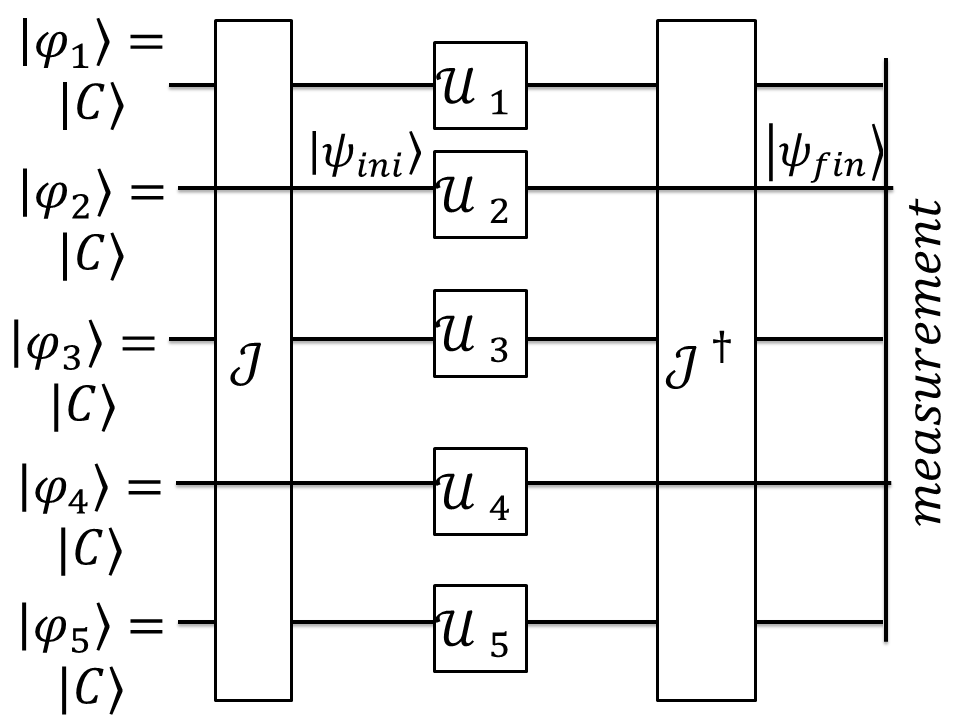
\includegraphics[scale=0.14]{Figures/architecture/esquema/esquema.png}
\caption{Scheme that represents the set-up of the $3$-player Pirate Game. Before we measure the final result we need to apply the transpose operator $\mathcal{J}^{\dagger}$. }
\label{fig:pg_architecture3players}
\end{figure}








\section{Analysis and Results}
\label{sec:description_3}


In order to test our model we developed a Matlab simulation for the $2$-player version of the game and for the $3$-player version, the simulations are available in the Appendix \ref{ap:d}. When defining our game space $\Gamma$ in Section \ref{subsec:pirates_initialstate} we defined a number of variable parameters, such as: the entanglement coefitient $\gamma$; the coin distributions $\alpha_{ij}$; the strategies $\mathcal{U}_{j}$ that the players might use (restricting the operator space $\mathsf{SU}(2)$).

According to \cite{Du} when the entanglement is maximal, $\mathcal{U}(\pi, 0)$ is the optimal counter-strategy for $C$ (represented by the identity marix), $\mathcal{U}(0, \frac{\pi}{2})$ is the optimal counter strategy for $\mathcal{U}(\pi, 0)$, $D$ becomes the optimal counter-strategy for $\mathcal{U}(0, \frac{\pi}{2})$, and $C$ becomes an optimal counter strategy for $D$. 

\subsection{$2$ Player Game}
\label{subsec:2playergame}

We simulated the Pirate Game for $2$-players according to the rules defined for our quantum model in Section . The simulation can be consulted for reference in Appendix \ref{ap:d}. The classical sub-game with $2$-players can be represented in Table \ref{tab:classico2jogadores_analise}. It is a strictly determined game, that means that there is at least a Nash Equilibrium when the players choose pure strategies\cite{Leyton-Brown2008:Essentials_Game_Theory}. In this case the outcome of the game is $(100, 0)$, when the players, use the strategies $C_{1}$ and $D_{2}$.  In the quantum game we can find the following $4$ pure quantum strategies :

\begin{itemize}

\item $I$

\item $D$ (also a Pauli operator $\sigma_{x}$)

\item $\mathcal{U}( \pi, 0)$ - a quantum equivalent of a defection operator, (also $i \sigma_y$).

\item $\mathcal{U}( 0, \frac{\pi}{2})$ - the quantum equivalent of a cooperation operator, (also $i \sigma_z$).

\end{itemize}

The expected utility when players can choose only pure quantum strategies and the game is maximaly entangled is shown in Figures \ref{fig:pg_2players_99_0_1:1} and \ref{fig:pg_2players_99_0_1:2}. When each player has access to the $4$ quantum strategies and the entanglement is maximum ($\gamma=\frac{\pi}{2}$), the game is not strictly determined anymore. The mixed strategy will make the players choose with equal probability between the 4 pure quantum strategies described above giving the players an expected payoff of $(25, 25.125)$, this outcome constitutes a Pareto optimal outcome because it is impossible to improve one player's expected utility without lowering the other's. 

As there were initialy 100 coins we decided to study what would happen if the captain decided to share the treasure fairly: $50$ coins for player $1$, $50$ for player $2$. A Nash equilibrium of the game would also consist in a mixed strategy where the players would choose indiferently which strategy to use, but in this case $\frac{3}{4}$ of the time player $1$ would get $50$ coins and $\frac{1}{4}$ he would die and receive a payoff of $-200$. This means that the meek captain would rather have a division ``supervised'' by a contract (entanglement), than to trust her crew and propose a fair division from the start.

\begin{table}[h]
\begin{center}
\begin{centering}
\begin{tabular}{ccc}
\hline 
  & Player 2: C & Player 2: D\tabularnewline
\hline 
Player 1: C & (100, 0) & (100, 0)\tabularnewline
Player 1: D & (100, 0) & (-200, 100.5)\tabularnewline
\hline 
\end{tabular}

\par\end{centering}
\caption{Representation of the $2$ player sub-game in normal form.}
\label{tab:classico2jogadores_analise}
\end{center}
\end{table}

\begin{figure}[h!]
\centering 
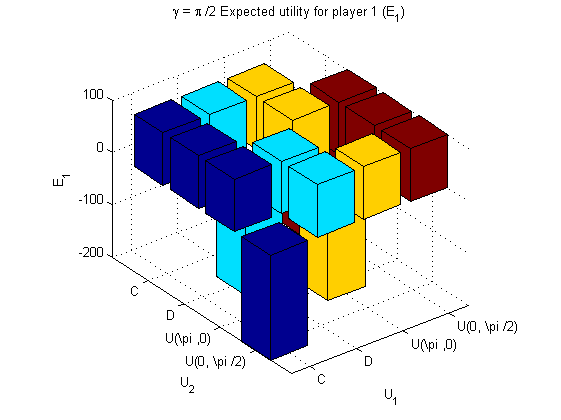
\includegraphics[scale=0.60]{Figures/1.5qubit/p2_E1.png}
\caption{Expected utility for player $1$, when both players have access to pure quantum strategies and the entanglement is maximum. }
\label{fig:pg_2players_99_0_1:1}
\end{figure}

\begin{figure}[h!]
\centering 
\includegraphics[scale=0.60]{Figures/1.5qubit/P2_E2.png}
\caption{Expected utility for player $2$, when both players have access to pure quantum strategies and the entanglement is maximum. }
\label{fig:pg_2players_99_0_1:2}
\end{figure}



\begin{figure}[h!]
\centering 
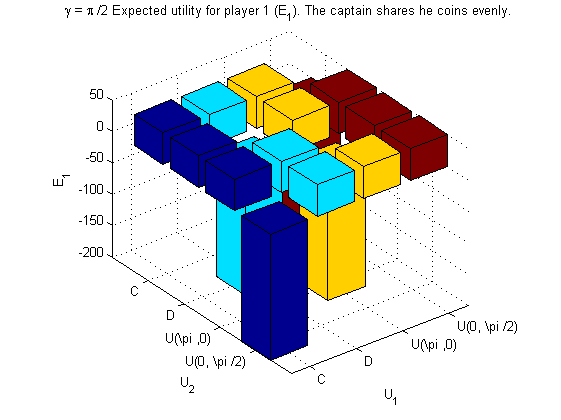
\includegraphics[scale=0.60]{Figures/1.5qubit/poorcaptain.png}
\caption{Expected utility for player $1$ (the captain), when the system is maximaly entangled and he proposes a fair division of the treasure $(50,50)$.}
\label{fig:pg_2players_99_0_1:33}
\end{figure}


\begin{figure}[h!]
\centering 
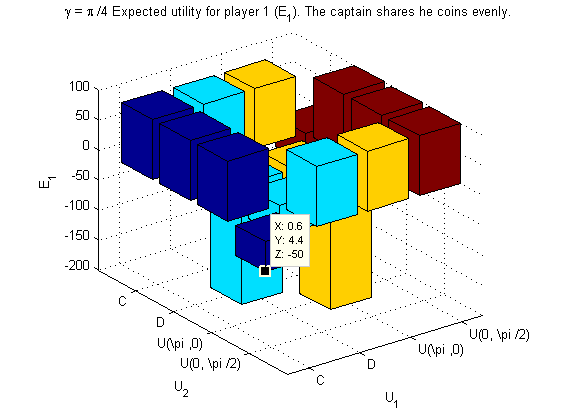
\includegraphics[scale=0.60]{Figures/1.5qubit/piadividirpor4.png}
\caption{Expected utility for player $1$ (the captain), when the entanglemet coefficient is $\gamma=\frac{\pi}{4}$ and he proposes a division of the treasure of $(100,0)$.}
\label{fig:pg_2players_99_0_1:33jesus}
\end{figure}

\subsection{$3$ Player Game}
\label{subsec:3playergame}


\subsubsection{The captain proposes: $(99, 0, 1)$}
\label{subsubsec:3playergame99}

The move $(C_1,D_2,C_3,C_4,D_5)$ with a proposal of $(\alpha_{1}, \alpha_{2}, \alpha_{3}) =(99, 0, 1)$ represents Nash Equilibrium of the classic Pirate Game (for $3$ players). In the classical version, when the players chose at least $2$ operators $Cooperate$ on the initial proposal the game ends right away, and the first proposal, made by player $1$, is accepted ($Accepted 1$ or $A_{1}$). Once again the original version of this game game is a strictly determined game because it has a pure-strategy Nash Equilibrium.

After the players make their strategic moves and the disentangle operator $\mathcal{J}^{\dagger}$ is applied, and the payoff functionals are calculated given the final state. The final state will be calculated as shown in Equation \eqref{eq:piratas_final_move_23}.

\begin{equation}
\vert\psi_{fin}\rangle=\otimes_{i=1}^{3}\otimes_{j\in\xi^{-1}(i)}\mathcal{U}_{j}\vert\psi_{ini}(\gamma)\rangle
\label{eq:piratas_final_move_23}
\end{equation} 

As expected from the problem definition when players use only classical strategies the entanglement coefficient will not affect the final expected utilities ($[ \mathcal{J} , C \otimes D \otimes C \otimes C \otimes D ] = 0 $).
An example of this behaviour is shown in Figure \ref{fig:pg_3players_99_0_1}, where we measure the probability $A_{1}$ (first proposal is accepted), $A_{2}$, and $R_{2}$, with different entanglement levels ($\gamma= \{ 0 , \frac{ \pi}{4}, \frac{\pi}{2} \} $).

\begin{figure}[h!]
\centering 
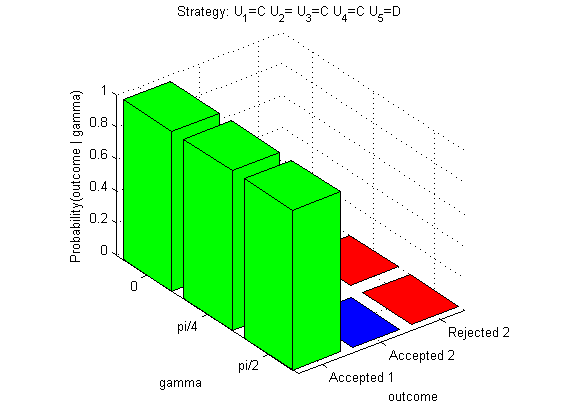
\includegraphics[scale=0.80]{Figures/1.5qubit/CDCCD.png}
\caption{When player play classical strategies the entanglement will not affect the final result. }
\label{fig:pg_3players_99_0_1}
\end{figure}

When each player chooses an operator from the set $O = \{ \mathcal{U} ( \theta , 0) , \theta \in (0, \pi) \}$ and $\gamma=0$ we have a separable game. This is an aquivalent situation to the classical game, but contrarily to the classical game where we have only a Nash Equilibrium $(C,D,C,C,D)$, we have more Equilibria, all with an outcome of $(99, 0, 1)$. This is verifyable because in the separable game the players act only in their qubits $\varphi_{j}$, and $D\vert 0\langle =\vert 1 \langle$ and $\mathcal{U}( \pi, 0) \vert 0 \rangle = - \vert 1 \rangle $, when measuring the probability of the operators $D$ and $\mathcal{U}( \pi, 0)$ tranforming a pure state $\vert 0 \rangle$ into state $\vert 1 \rangle$ we square the probability amplitude associated with the final state. When $\gamma = 0$  $C$ is interchangeble with $\mathcal{U}(0, \frac{\pi}{2})$, and $D$ is interchangeble wih $\mathcal{U}( \pi, 0)$.

However for $\gamma >0$ the $\mathcal{U} ( \theta , 0)$ may present an interference behaviour that is inherently quantum. This effect is shown in Figures \ref{fig:pg_3players_99_0_1:2} and \ref{fig:pg_3players_99_0_1:2}, allowing us to understand the difference between the Bit-flip operator $D$ and $\mathcal{U} ( \pi , 0)$.



\begin{figure}[!h]
\centering 
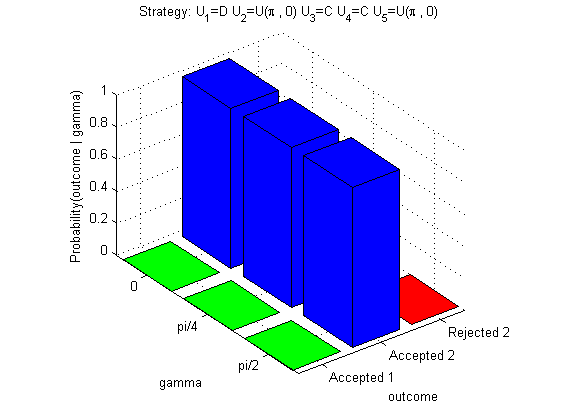
\includegraphics[scale=0.80]{Figures/1.5qubit/DUpi0CCUpi0.png}
\caption{Players use the operators . }
\label{fig:pg_3players_99_0_1:2}
\end{figure}

\begin{figure}[h!]
\centering 
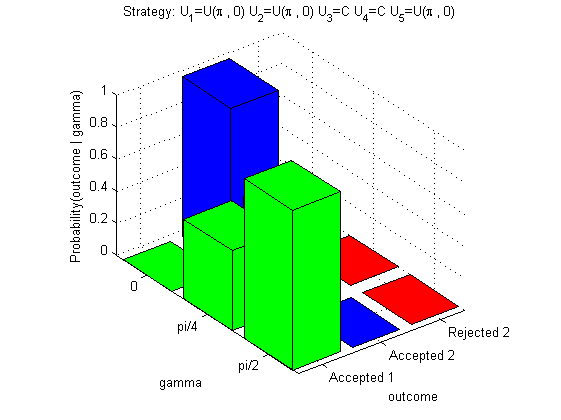
\includegraphics[scale=0.80]{Figures/1.5qubit/Upi0Upi0CCUpi0.png}
\caption{Unlike with the Bit-flip operator $D$, $\mathcal{U} (\pi, 0)$ is affected by the entanglement coefficient $\gamma$ in this case. }
\label{fig:pg_3players_99_0_1:3}
\end{figure}


The Tables \ref{iamlivingontheedge} and \ref{livingontheedge} represent a $3$-player pirate game where given the classical equilibrium $(CDCCD)$ we test what are the outcomes if the players can use quantum strategies. By considering the quantum operators that constitute an alternative to the classical cooperation ( $\mathcal{U}( 0, \frac{\pi}{2})$ ), or defection ( $\mathcal{U}( \pi, 0)$ ), like in the $2$-player analysis when the entanglement is maximum we found that there is only a mixed strategy Nash Equilibrium because we detect a restricted cycled as suggested by \cite{Du}. 

%The player $1$ (the first captain), should play half the time the classical cooperation matrix (the identity matrix)), the other half the operator $\mathcal{U}( 0, \frac{\pi}{2})$. 


\begin{center}
\begin{table}
\begin{centering}
\begin{tabular}{ccc}
\hline 
 & Player 3: $\tau_{3}=\{C,D\}$ &  $\tau_{3}=\{C,\mathcal{U}(\pi,0)\}$\tabularnewline
\hline 
Player 2: $\tau_{2}=\{D,C\}$ & (99,0,1) & (-200,100.5,0.5)\tabularnewline
$\tau_{2}=\{D,\mathcal{U}(0,\frac{\pi}{2})\}$ & (-200,100.5,0.5) & (99,0,1)\tabularnewline
$\tau_{2}=\{\mathcal{U}(\pi,0),C\}$ & (-200,100.5,0.5) & (99,0,1)\tabularnewline
$\tau_{2}=\{\mathcal{U}(\pi,0),\mathcal{U}(0,\frac{\pi}{2})\}$ & (99,0,1) & (-200,100.5,0.5)\tabularnewline
\hline 
\hline 
 & $\tau_{3}=\{\mathcal{U}(0,\frac{\pi}{2}),D\}$ & $\tau_{3}=\{\mathcal{U}(0,\frac{\pi}{2}),\mathcal{U}(\pi,0)\}$\tabularnewline
Player 2: $\tau_{2}=\{D,C\}$ & (99,0,1) & (-200,100.5,0.5)\tabularnewline
$\tau_{2}=\{D,\mathcal{U}(0,\frac{\pi}{2})\}$ & (-200,-199.5,100.5) & (99,0,1)\tabularnewline
$\tau_{2}=\{\mathcal{U}(\pi,0),C\}$ & (-200,100.5,0.5) & (99,0,1)\tabularnewline
$\tau_{2}=\{\mathcal{U}(\pi,0),\mathcal{U}(0,\frac{\pi}{2})\}$ & (99,0,1) & (-200,-199.5,100.5)\tabularnewline
\end{tabular}
\par\end{centering}
\caption{Player 1 plays C. $\tau_{i}$ represents the player $i$'s strategy, by assigning an operator to the qubits that she controls. $\gamma=\frac{\pi}{2}$. The first captain proposes the following distribution $(99,0,1)$; the second captain proposes $(100,0)$. }
\label{iamlivingontheedge}
\end{table}

\par\end{center}


\begin{center}
\begin{table}[h!]
\begin{centering}
\begin{tabular}{ccc}
\hline 
 & Player 3: $\tau_{3}=\{C,D\}$ &  $\tau_{3}=\{C,\mathcal{U}(\pi,0)\}$\tabularnewline
\hline 
Player 2: $\tau_{2}=\{D,C\}$ & (99,0,1) & (-200,100.5,0.5)\tabularnewline
$\tau_{2}=\{D,\mathcal{U}(0,\frac{\pi}{2})\}$ & (-200,-199.5,100.5) & (99,0,1)\tabularnewline
$\tau_{2}=\{\mathcal{U}(\pi,0),C\}$ & (-200,100.5,0.5) & (99,0,1)\tabularnewline
$\tau_{2}=\{\mathcal{U}(\pi,0),\mathcal{U}(0,\frac{\pi}{2})\}$ & (99,0,1) & (-200,-199.5,100.5)\tabularnewline
\hline 
\hline 
 & $\tau_{3}=\{\mathcal{U}(0,\frac{\pi}{2}),D\}$ & $\tau_{3}=\{\mathcal{U}(0,\frac{\pi}{2}),\mathcal{U}(\pi,0)\}$\tabularnewline
Player 2: $\tau_{2}=\{D,C\}$ & (-200,100.5,0.5) & (99,0,1)\tabularnewline
$\tau_{2}=\{D,\mathcal{U}(0,\frac{\pi}{2})\}$ & (99,0,1) & (-200,-199.5,100.5)\tabularnewline
$\tau_{2}=\{\mathcal{U}(\pi,0),C\}$ & (99,0,1) & (-200,100.5,0.5)\tabularnewline
$\tau_{2}=\{\mathcal{U}(\pi,0),\mathcal{U}(0,\frac{\pi}{2})\}$ & (-200,-199.5,100.5) & (99,0,1)\tabularnewline
\end{tabular}
\par\end{centering}

\caption{Player 1 plays $\mathcal{U}(0,\frac{\pi}{2})$.$\gamma=\frac{\pi}{2}$. The first captain proposes the following distribution $(99,0,1)$; the second captain proposes $(100,0)$. }
\label{livingontheedge}
\end{table}

\par\end{center}



\subsubsection{The captain proposes: $(100, 0, 0)$}
\label{subsubsec:3playergame100}

Suppose captain is greedy and proposes to get the 100 coins. In the classical Pirate Game this would pose a conflict with his self-preserving needs. 
A pertinent question would be if this Quantum Model of the Pirate Game would allow the first captain to approve that allocation proposal. 

If the captain is the only one with access to quantum strategies, and the other players do not know it and play the classical strategies $C$ (identity matrix) and $D$ (Bit-flip operator), there is a dominant quantum strategy that allows her to pass her proposal and get all the $100$ coins, for $\gamma = \frac{\pi}{2}$. Figure \ref{fig:pg_3players_99_0_1:4} provides an example that corroborates where we verify that player $1$ has a set of dominant strategies (for $\tau_{1} = \mathcal{U}_{1}(\pi,\phi), \phi \in (0, \frac{\pi}{2})$ or $\tau_{1} = \mathcal{U}_{1}(\theta,\frac{\pi}{2}), \theta \in (0, \pi)$). We verified experimentally that the sub-games with $2$ players (when $(C_{4},C_{5}), (C_{4},D_{5}), (D_{4},C_{5}), (D_{4},D_{5})$), did not affect this dominant strategy. If fact if we analyse the expected utility function for player $1$ ($E_{1}.$), and the Figure \ref{fig:pg_architecturegametree:extensiveform} representing the extensive form game, we verify that the the first captain is indifferent to the results of the sub-game with $2$-players, when both player play a classical strategy, because she is already dead. 

\begin{figure}[h!]
\centering 
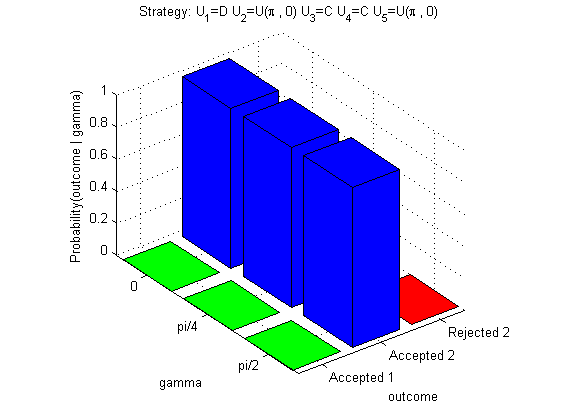
\includegraphics[scale=0.80]{Figures/1.5qubit/DUpi0CCUpi0.png}
\caption{Player $1$ uses the classical operator D. The probabilities don't change with the entanglement.  }
\label{fig:pg_3players_99_0_1:2}
\end{figure}

\begin{figure}[h!]
\centering 
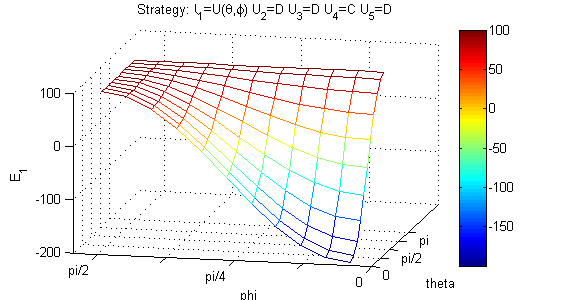
\includegraphics[scale=0.80]{Figures/1.5qubit/meanpirate.png}
\caption{Expected utility for player $1$ when she adopts a strategic move of the form $U_{1}(\theta,\phi)$ and the other players play $D_{2},D_{3},C_{4},D_{5}$. }
\label{fig:pg_3players_99_0_1:4}
\end{figure}

If players $2$ and $3$ know that the captain has access to quantum strategies, with a maximaly entangled game, and they have the restricted sub-set of pure classical strategies $C_{j}$ and $D_{j}$, if they both play $C$, the dominant strategy for the captain becomes $\tau_{1} = \mathcal{U}_{1}(0,0)$. Their best response becomes playing a mixed strategy where half the time they will play $C$ and the other half $D$. The best response for player $1$ in this case is to play a mixed quantum strategy where half the time she plays $\mathcal{U}(0,0)$, half $\mathcal{U}(0,pi/2)$.



\begin{figure}[h!]
\centering 
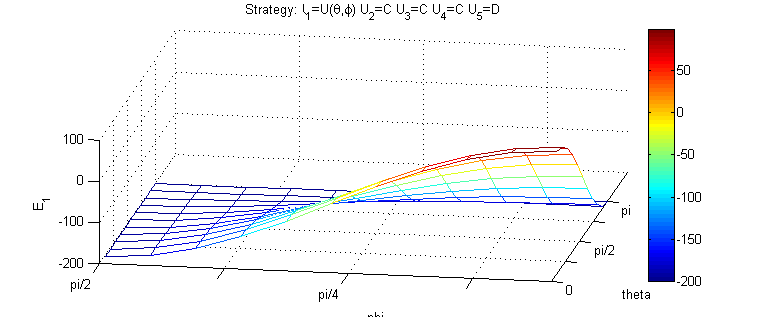
\includegraphics[scale=0.80]{Figures/1.5qubit/meanpirategetscrewed.png}
\caption{Players $2$ and $3$ use a mixed classical strategy to choose the operators $O_{2}$ and $O_{3}$, where half the time they will play $C$ and the other half $D$. }
\label{fig:pg_3players_99_0_1:2}
\end{figure}

\begin{figure}[h!]
\centering 
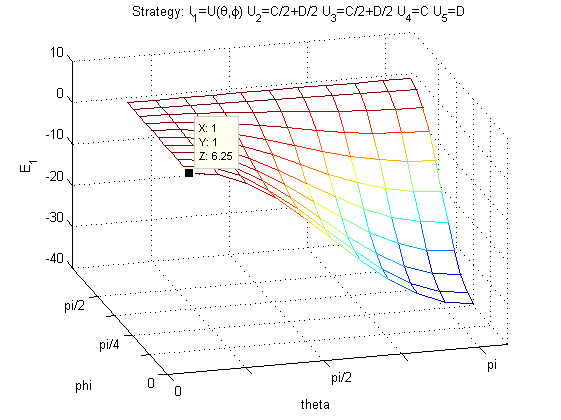
\includegraphics[scale=0.80]{Figures/1.5qubit/mixedclassical.png}
\caption{Players $2$ and $3$ use the operators $C_{2}$ and $C_{3}$. }
\label{fig:pg_3players_99_0_1:2}
\end{figure}

\begin{figure}[h!]
\centering 
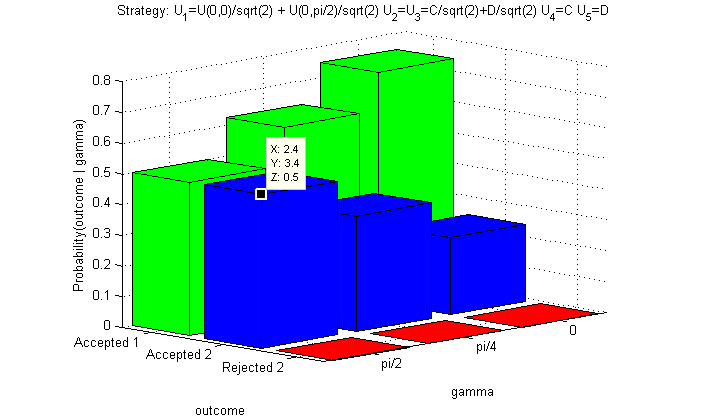
\includegraphics[scale=0.80]{Figures/1.5qubit/mixedmixedclassical.png}
\caption{Players $2$ and $3$ use the operators $C_{2}$ and $C_{3}$. }
\label{fig:pg_3players_99_0_1:2}
\end{figure}






\section{Conclusion}


We tried to get our Quantum Model of the Pirate Game as close as possible in order to compare the the original game. However we did not incorporate the concept of measuring the results between rounds of voting. In the original problem after each stage the results are accounted. Our approach was deemed more adequate to analyse in \cite{Fra2011}.

In works such as the Prisoner's Dilemma\cite{Letters2002}\cite{Eisert2008}, and Quantum Ultimatum Game\cite{Fra2011}, the strategic space was analysed allowing a infinity of mixed quantum strategies. Our game space was much more vast than the works previously mencioned, we used $5$ qubits to model our system, their models had no more than $3$ qubits. This imposed that in order to analyse our system while conceptualy, our strategic space is also infinite, we restricted in order to analyse. In particular we payed special interest in the strategies: $C$, $D$, $\mathcal{U}(\pi, 0)$, and $\mathcal{U}(0, \frac{\pi}{2})$. The first two mensioned strategies are the equivalent of the classical strategies ``Cooperate'' and ``Defect'', the other two are quantum strategies. Toghether these $4$ strategies when paired with the coefitients $(w,x,y,z)$ are known to span a class that contains all unitary operators, the $\mathsf{SU}(2)$. According to \cite{Du} these $4$ operators when the entanglement is maximum provided a cycle where each operator was an optimal counter strategy to other. 

The set-up of the initial system was crucial to introduce the phenomenon of entanglement. We concluded that without entanglement the game has a strictly determined solution and behaves as the original problem, however there are more pure strategy Nash Equilibria.

For the $2$-player game we concluded that the expected utility when the players use a mixed strategy Nash equilibrium renders an expected utility of $(25, 25.125)$ wich is also a Pareto optimal solution because it is not possible to improve one player's expected utility without harm the other. The classical setting is more beneficial to the captain in this game, because she will receive the 100 coins. We also found that distributing 50 coins would give a lower expected utility to the captain. This result is interesting because it is a Pareto optimal solution in the classical version, though not a Nash Equilibrium, and it renders an higher payoff than the Nash Equilibrium and Pareto Optimal solution when the sytem is maximaly entangled and the players have access to the $4$ pure quantum strategies discussed in \cite{Du} and \cite{Letters2002}. 

The $3$-player game also has a mixed quantum strategy Nash Equilibrium, like the $2$-player game, when the entanglement is maximum, however its calculus fell beyond the scope of this dissertation. 

When trying to find if it is possible for the captain in the first stage of the game to acquire all gold coins we found that if the other players have a restricted set of strategies, they can only use the classical Cooperate or Defect operators, and if they don't know that the captain has access to quantum strategies, the captain will be able to get the $100$ gold coins. However if players $2$ and $3$ have a restricted set where they can only use the classical Cooperation operator, or the classical Defection operator, the player $1$ will no longer be able to acquire the 100 coins with certainty. Instead she may be able to acquire the $100$ coins with probability $\frac{1}{2}$ or end up thrown off board with equal probability.

These results corroborate the literature in the Chapter 3, while contributing with another case study.

 
 






%\bibliographystyle{IEEEtran}
%\bibliographystyle{splncs}
%\bibliographystyle{ieeetr}
%\bibliography{02.biblio}

\bibliographystyle{IEEEtran}
\bibliography{02.biblio}



\end{document}
